\chapter{Lines detection}
\label{Chap:LineDetect}


%-----------------------------------------------------------------------
%-----------------------------------------------------------------------
%-----------------------------------------------------------------------

\section{Introduction}

%-----------------------------------------------------------------------

\subsection{Context and scope}

This chapter describes the method developped for line detection in \PPP. 
These methods have been developed in the case of wire detection in the context
of collaboration with CERN for magnet alignment.

At the time being, the method and describtion is  higly oriented to this use case,
in fact it is more or less limited to this case for now  but the different elementary
part could be easily re-used to process more general cases. This chapter mixes
algorithmic specification, developer and end-user .


%-----------------------------------------------------------------------
\subsection{Overview of the method}

The main steps of line detection are the following :

\begin{itemize}
    \item {\bf Image Space computation}
         \begin{itemize}
              \item compute de gradient of image 
              \item extract the local maxima of gradient, in the direction of gradient
              \item refine de position  (transform integer pixel coordinate in refined real coordinates);
         \end{itemize}
    \item {\bf Hough space computaion}
         \begin{itemize}
             \item compute the hough transform  (at this step, each wire generate two \emph{anti parallel} lines);
             \item extract the local maxima in hough space , in integer coordinates, and refined them, 
         \end{itemize}

    \item {\bf Back to image space computation}
         \begin{itemize}
             \item \emph{back transformate} hough point in line, and refine their coordinate using the initial gradient point;
             \item match the lines for computing pairs of antiparallel lines, and extract caracteristic of central lines
                   including quality criteria (parallelism, width, radiometric homogeneity);
             \item select the \emph{best} lines by comparison of quality criteria.
         \end{itemize}
\end{itemize}

In the process we have to take into account image distorsion, because this in \emph{un-distorded} coordinates,
that the wire is a straight line. As we dont want to make an image ressampling
\footnote{because it cannot be used with fish-eye and limit the image quality} , all along the process we
will have to make frequent back and forth between initial and undistorted coorinates.  For the sake
of simplicity, we will no longer mention them here.

%-----------------------------------------------------------------------
\subsection{Localisation of the code}

The command for extracting line is {\tt ExtractLine}, the code of the command is
located in {\tt cAppliExtractLine.cpp}.  The algorithms used in this command,
can mainly be found in the folder {\tt src/ImagesInfoExtract} :

\begin{itemize}
    \item  {\tt cImGradWithN.cpp}  code for computing gradient (sobel, deriche),
           the method calls some code of file {\tt include/MMVII\_TplGradImFilter.h};


    \item  {\tt cHoughTransform.cpp}  code for computing the hough transform

    \item  {\tt cAppliExtractLine.cpp}, code for extracting lines, calling previous
           facilities (gradient, hough );
\end{itemize}

%-----------------------------------------------------------------------
%-----------------------------------------------------------------------
%-----------------------------------------------------------------------

\section{Computation in image space}

\subsection{Compute de gradient of image}
There is  $2$ option for computing the gradient :

\begin{itemize}
    \item   the \emph{Deriche} gradient
    \item   the \emph{Sobel} gradient
\end{itemize}

The sobel method is significantly faster, and apparently gives equivalent result for our purpose
\footnote{consquently, for now  the deriche variant is no longer completely supported}.
The method for computing \emph{Sobel} filter can be found in {\tt MMVII\_TplGradImFilter.h}.

Also basic implementation of \emph{Sobel}  is quite obvious,  some precaution have been
taken for making it as effeciency as possible.  The low level optimized services are offered
in  class {\tt cTabulateGrad} :

\begin{itemize}
    \item  for fast computing of norm of gradient, its value is computed
           for any possible value of $G_x,G_y$ and stored in a table
           (for example a $256 \times 256$ table if we know that $G_x, G_y \in [128,-128[^2 $);

    \item  {\tt cTabulateGrad(int aVMax);} is the constructor, the $aVMax$ value
          is used to limit the number of possible values in tabulation;

    \item  the method {\tt ComputeSobel} store in $2$ image $G_x$ and $G_y$ the value
           of gradient in $x$ and $y$;  it takes a parameter {\tt Div} for dynamic of
           storing, all values of $G_x,G_y$ are divied by {\tt Div}.

\end{itemize}

Figure~\ref{Fig:Line:Grad} present the result of \emph{Sobel} gradient on a small image
containing a wire.


\begin{figure}
\centering
        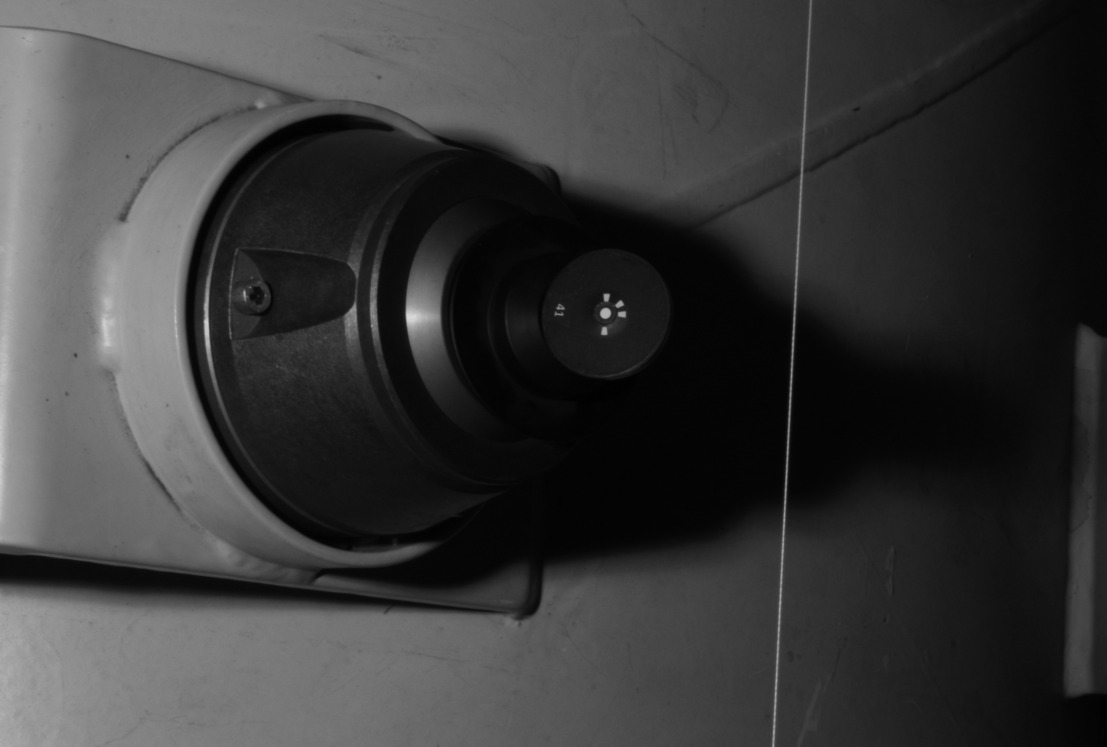
\includegraphics[width=4cm]{Methods/ImagesFils/ImagOri.jpg }
        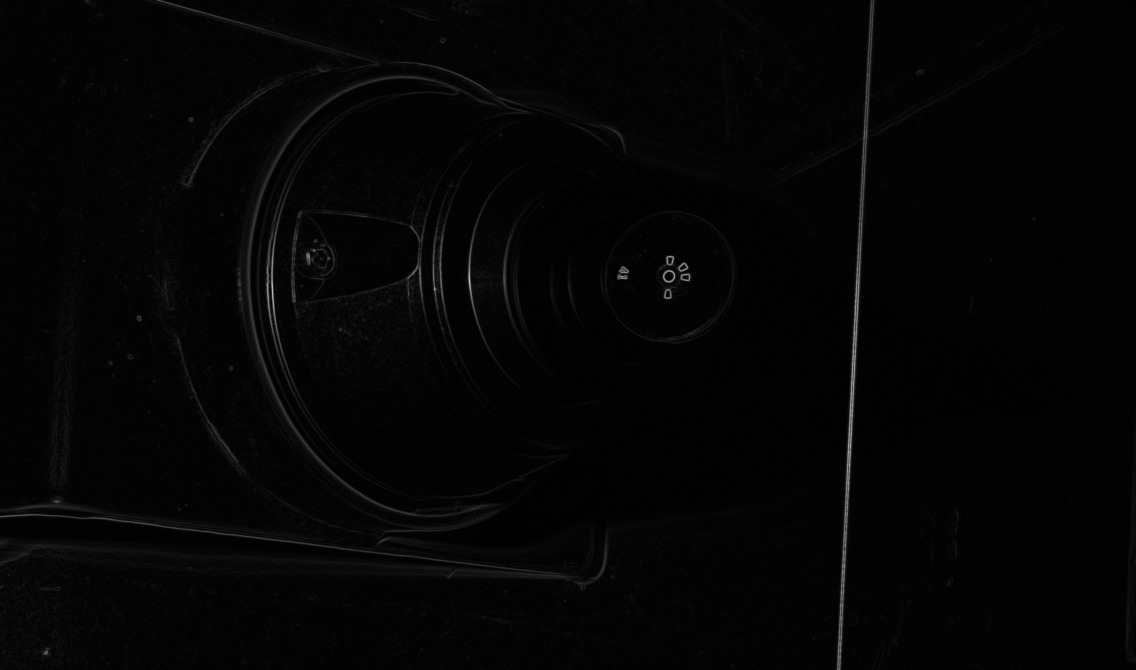
\includegraphics[width=4cm]{Methods/ImagesFils/GradInit.jpg }
        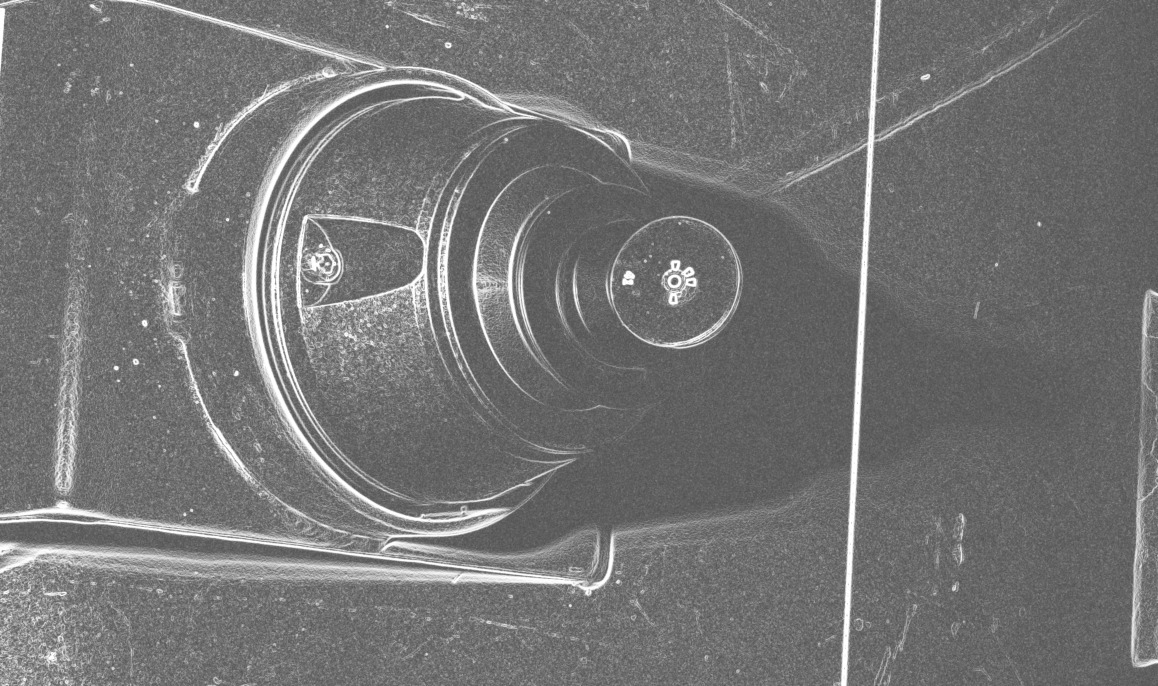
\includegraphics[width=4cm]{Methods/ImagesFils/GradNonLinear.jpg }
        \caption{An extract of image, the sobel gradient, non linear radiometric enhance of gradient}
\label{Fig:Line:Grad}
\end{figure}

%-----------------------------------------------------------------------

\subsection{Selection of local maxima of gradient}

\label{Line:LocMaxGrad}

Extracting the local maxima of the gradient in the direction of gradient is a very classical pre-processing
in computation of  edge detection.  But there is some precuation  to tack into account here because :

\begin{itemize}
   \item on want side we want to select point that are maxima on sufficiently large neighboorhoud
         to have an efficient pre-filter (the point selected will be used for hough transform which
         can be relatively long);

   \item on the other side, we must tacke into account that for each line we want to detect, there exist 
        a close anti-parallel line, that will have a module of gradient comparable; due to noise,
        sampling, background, this anti parallel line may eliminate the point.
\end{itemize}

To avoid elimination of many points by their macthing anti parallel line, we proceed this way,
illustrated by left schema of figure~\ref{Fig:Line:MaxLocGrad} :

\begin{itemize}
   \item let  $P$ be a pixel of image were gradient is $\vec G$

   \item  $\rho_0$ and $\rho_1$ be two thresholds, low and hig, of size of
          and $\theta$ be angular threshold
           (value  $\rho_0=1$, $\rho_1=8$ and $\theta=\frac{\pi}{2}$ are used in {\tt ExtractLine})

   \item  we define $N_1$  the neighbourhoud defined by point $Q$ with $\vec u = \overrightarrow{PQ}$ such
          that  $ < \rho_1$  and $ | \widehat{\vec G \vec{u}} | < \frac{\theta}{2}  $

   \item idem for $N_0$


   \item we define also $N_1^+$  by  $N_1^+ = \{Q \in N_1 / \vec u . \vec G >0\} $
          (and similarly $<0$ for $N_1^-$).
          \footnote{if the the wire is  black, instide of white, the definition
           of $N_1 ^-$ and $N_1 ^+$ are swapped}

\end{itemize}

Now, to select  a point as a local maxima of the gradient we require that the following condition are
all satisfied :

\begin{itemize}
    \item  $|\vec G(P)|  \gg  |\vec G(Q)|  \forall  Q \in N_0$ , in the  \emph{small} neighbourhood , there is no risk
           to meet the anti-parallel line;

    \item  $|\vec G(P)|  \gg  |\vec G(Q)|  \forall  Q \in N_1 ^-$ in the direction opoposed to gradient, there is
           no risk to meet the anti-parallel line 

            
    \item  $ (|\vec G(P)|  \gg  |\vec G(Q)|)  or (\vec G(P) . \vec G(Q) <0 )    \forall  Q \in N_1 ^+$

\end{itemize}

Where the relation  $ |\vec G(P)|  \gg  |\vec G(Q)| $ stands for :

\begin{itemize} 
     \item  $|\vec G(P)|  > |\vec G(Q)| $  
     \item or $(|\vec G(P)|  == |\vec G(Q)|) and (x_P >x_Q) $ 
     \item or $(|\vec G(P)|  = |\vec G(Q)|) and (x_P =x_Q)  and (y_P=y_Q)$
\end{itemize} 

This definition is made so, for mathematicall consitency,  $\gg$  is a strict order relation.
The result of this selection is illustrated on left image of  figure~\ref{Fig:Line:MaxLocGrad}.

\begin{figure}
\centering
        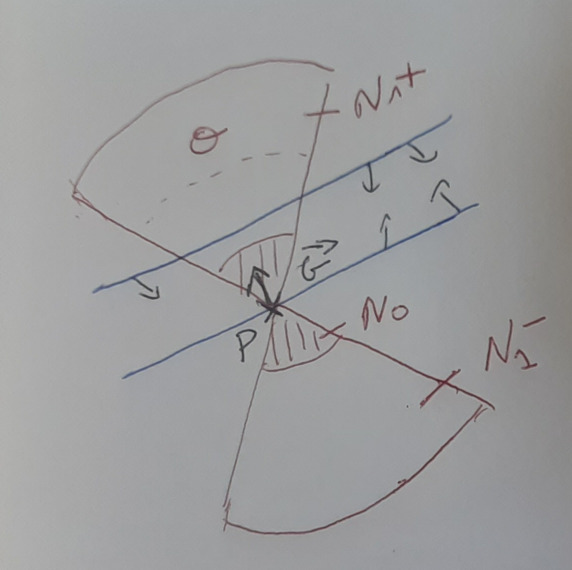
\includegraphics[width=6cm]{Methods/ImagesFils/NeighMaxLoc.jpg}
        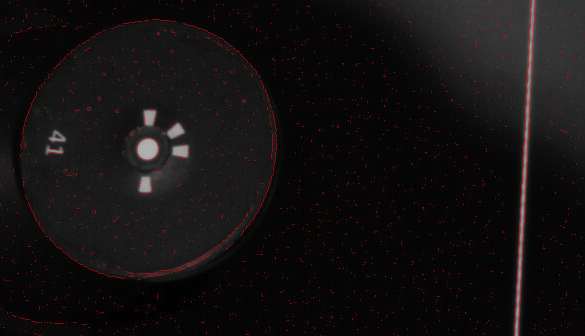
\includegraphics[width=6cm]{Methods/ImagesFils/MaxLocGrad.jpg}
        \caption{An extract of image, the sobel gradient, non linear radiometric enhance of gradient}
\label{Fig:Line:MaxLocGrad}
\end{figure}

On the tested images, with the used parameters, the proportion of pixels selected by this
procedure is less than $2\%$ of the initial set of pixels.


%-----------------------------------------------------------------------

\subsection{Refinement of local maxima}
\label{Ref:Grad:Loc:Max}

The previous selection return a set of pixels with integer coordinates, to have a better accuracy
their coordinates are then refined. The method used is the following , let:

\begin{itemize}
     \item  $\vec g =  \frac{\vec G}{|G|} $ be the unitary vector in direction of gradient;

     \item   $G_{1} = |\vec G(P+\vec g)|$ the norm of gradient at $1$ pixel distance in direction of gradient;
     \item   $G_{-1} = |\vec G(P-\vec g)|$  and $G_0 = |\vec G(P)|$
\end{itemize}

Consider now the parabol $\mathcal {P}$  such that  : $\mathcal {P}(-1) = G_{-1} $ , $\mathcal {P}(0) = G_{0} $ ,
$\mathcal {P}(1) = G_{1} $. Except in degenerate case, this $\mathcal {P}$ has a single extremum , note it $a$, we
then set  $P_r = P+ a\vec g $ , where $P_r$ is the refined point. On this simple bases, there is several
modification :

\begin{itemize}
    \item if we are in the degenerate case, or if the extremum is a minima we dont do anything;
    \item if $|a| > 1 $ we dont do anything;
    \item we make several iteration of this process ($2$ in the current code).
\end{itemize}

The corresponding code can be found in the method {\tt cImGradWithN<Type>::RefinePos}.


\TOIMPROVE{ maybe  try a metho that dont use gradient and its interpolation, like method computing directly
            the gradent in the interpolation, with a derivale interpolator like sinc of cubic }

%-----------------------------------------------------------------------
%-----------------------------------------------------------------------
%-----------------------------------------------------------------------

\section{Computation in hough space}

%-----------------------------------------------------------------------

\subsection{Notation and reminder of the hough transform}

Let $x,y$  be the set of  pixel of the image.  Let $D$ be a line parametrized
by $\rho, \theta$,  such that :

\begin{equation}
     x,y \in D(\rho,\theta)   \Leftrightarrow  x \cos (\theta) + y \sin (\theta) = \rho  \label{Line:EqRadon}
\end{equation}

The hough-transform is used here for counting for each lines 
the number of points through which it passes . It's very similar to radon
transform, it's somewhat just an inversion of  the process :

\begin{itemize}
    \item in radon transform, we parse all the possible line,i we sample the  line
          and count the sum of the image (function ) on the line;

    \item in hough transform we parse all the pixel, and for each pixel we
          sum the function in accumulator $H$  on all the lines that pass trough the point ,
          for this we use equation \ref{Line:EqRadon} to make the incrementation
          of equation \ref{Line:EqHough}.
         
\end{itemize}

\begin{algorithm}
\caption{Hough incrementation of $H$  for $x,y$ with value $I$}\label{alg:hough}
\begin{algorithmic}
\State $K_t \gets NbT$ \Comment{$ NbT$ : number of sampling in teta}
\While{$K_t \neq 0$}
    \State $\theta  \gets  \frac{2 K_t \pi}{NbT} $
    \State $\rho \gets  x \cos(\theta) + y \sin(\theta)  $  \Comment{This is a comment}
    \State $H(\theta,\rho) += I$
\EndWhile
\end{algorithmic}
\end{algorithm}

%-----------------------------------------------------------------------

\subsection{Oriented hough transform}

In general case, hough transform is equivalent to radon transform and relatively
slow, if the image has a size $N \times N$ , the computation time is in $N^3$.
What make hough very popular is that it can be very efficient in the case where
for the majority of point  we have $I(x,y) =0 $, because in this case we dont
need to enter in the loop~\ref{alg:hough}.
This is more a less what we do  with the computation of local maxmima in \ref{Line:LocMaxGrad},
instead of executing \ref{alg:hough} for all pixel, we do it for only the few \% of pixel
that were selected as local maxima.

By the way, there is more to do, because when we compute the gradient we have not only
its module but also its direction $\alpha$, so it is coherent to suppose that if
a straight line of  Hough/Radon-coordinate $\rho,\theta$ pass by this point we have $\theta \approx \alpha$.
Note, that doing that we consider \emph{oriented} line where direction are defined $\equiv 2 \pi$
and not single line defined  $\equiv \pi$; which is rather an advantage  if we want to
extract both each line and its antiparallel homologous they become distant in Hough/Radon space. 

So for each point, in  algoritm~\ref{alg:hough},
due to estimation $\alpha$ of $\theta$, we can reduce the initial
interval $[0,2\pi]$  to  $[\alpha-\delta,\alpha+\delta]$ where $\delta$ is  
the estimation of incertitude .  In command {\tt ExtractLine}, the default value
is empirically set to $\delta=0.1$, which seem safe enough and lead to an acceleration
of factor $30$ of hough transform.


The code corresponding to algorithm~\ref{alg:hough} can be found in method  :
\begin{itemize}
  \item {\tt void  cHoughTransform::Quick\_AccumulatePtAndDir(const cPt2dr \& aPt,tREAL8 aTetaC,tREAL8 aWeight); }
  \item {\tt void  cHoughTransform::Accurate\_AccumulatePtAndDir(const cPt2dr \& aPt,tREAL8 aTetaC,tREAL8 aWeight); }

  \item  once we have sampled the different value of $\theta$ the formula~\ref{Line:EqRadon} gives a real value
         of $\rho$, which does not fit exactly on a pixel of acccumularor, in quick version we simply round
         to nearest integer, while in second we split it using linear interpolation; by default  {\tt ExtractLine}
         uses quick version.
\end{itemize}

The figure~\ref{Fig:Line:Hough} represent the typical  result  we obtain at this step.

\begin{figure}
\centering
        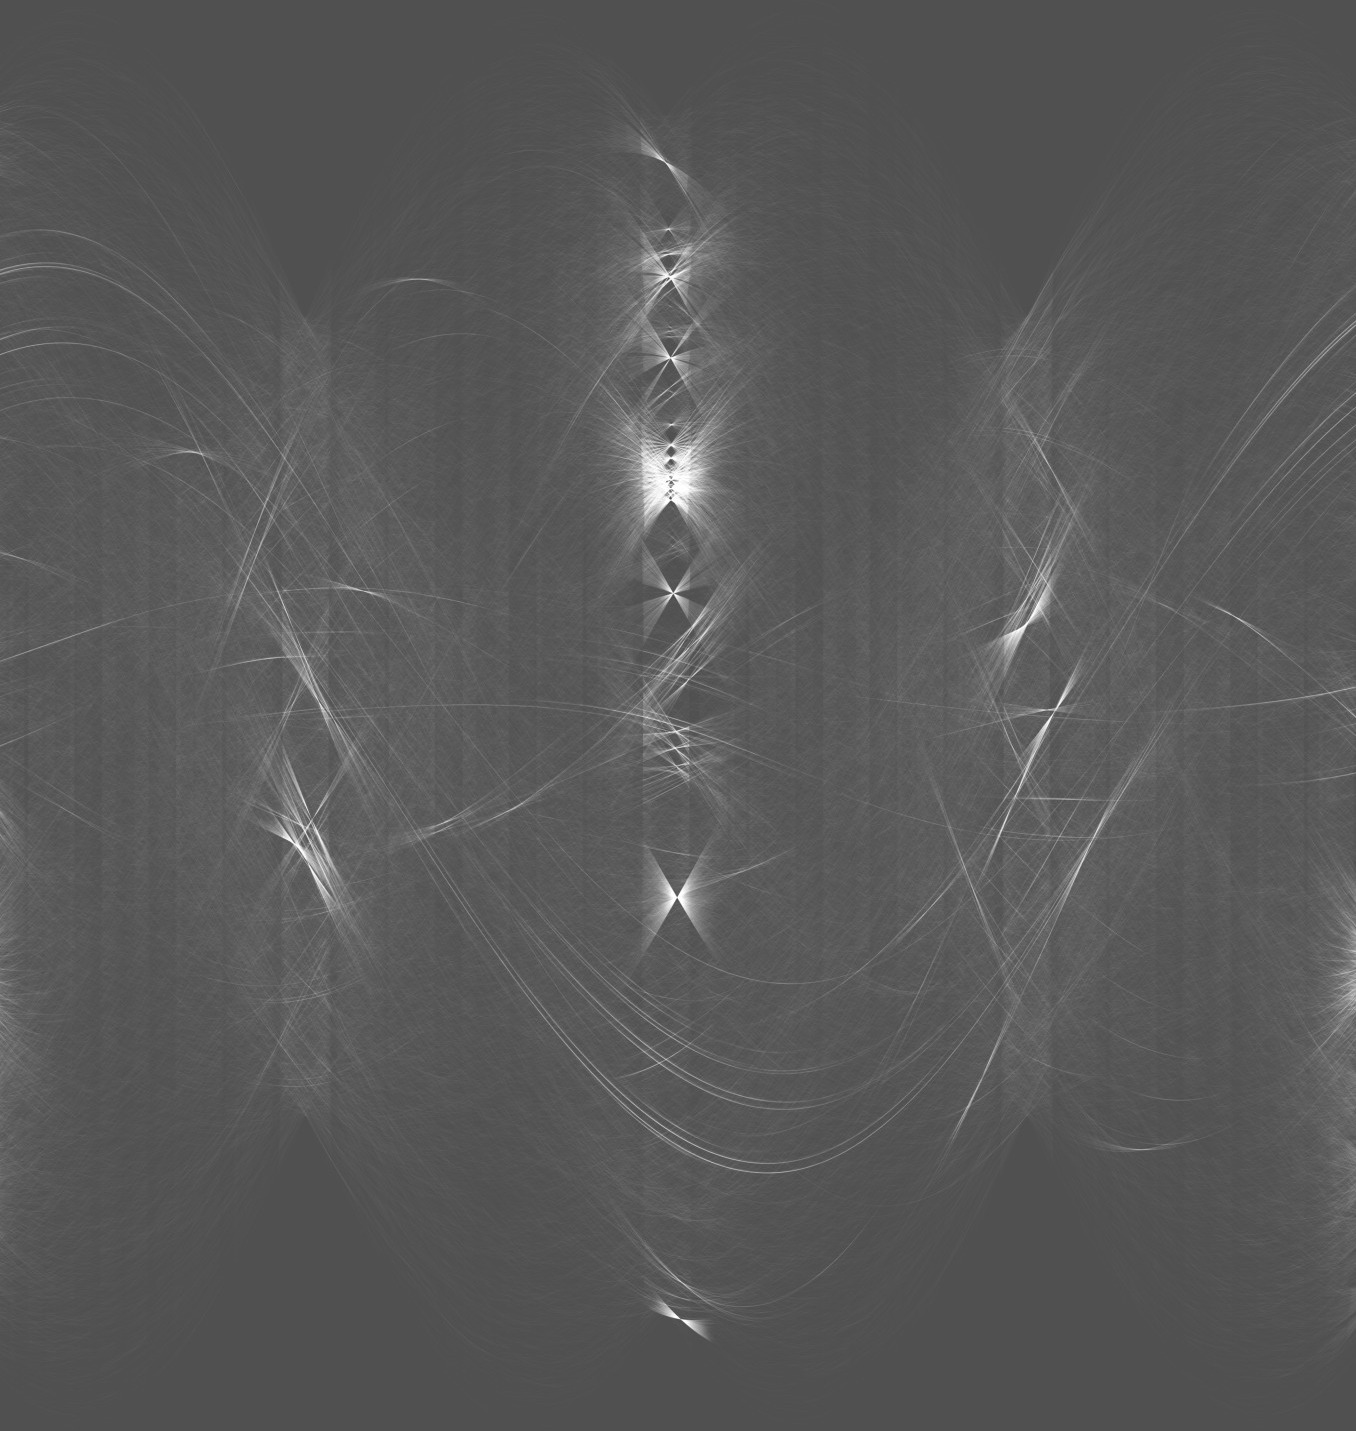
\includegraphics[width=8cm]{Methods/ImagesFils/FullHough.jpg}
        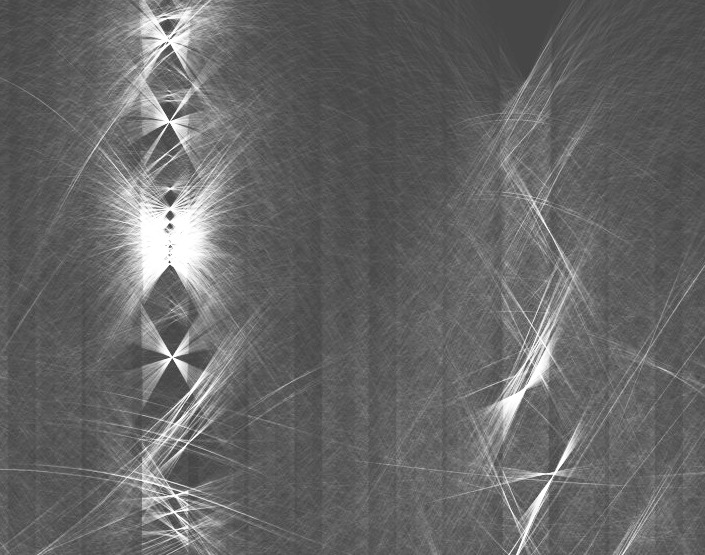
\includegraphics[width=8cm]{Methods/ImagesFils/Crop-Hough.jpg}
        \caption{Example of hough transform, and a crop on it}
\label{Fig:Line:Hough}
\end{figure}


%-----------------------------------------------------------------------

\subsection{Extraction of maxima of hough transform}

\label{Hough:Max:Loc}

The next step is to extract the "best" line candidate in hough space, 
this is done in  following steps :

\begin{itemize}
    \item  compute a threshold $Th$  taking into accound average $Avg_H$ and max $Max_H$ of hough accumulator,
           in current version $Th = \max (10*Avg, \frac{Max_H}{10})$
%    std::vector<cPt3dr> aVMaxLoc = mExtrL->Hough().ExtractLocalMax(10,5.0,10.0,0.1);
% std::vector<cPt3dr>  cHoughTransform::ExtractLocalMax(size_t aNbMax,tREAL8 aDist,tREAL8 aThrAvg,tREAL8 aThrMax) const
    \item  extract all the point for which $H(\rho,\theta) > Th$ and that are a local maxima in a 
           given neighbourhood, in current version of size of the neighbourhoud is $5$;

     \item once we  have selected the local maxima, we select if necessary the $K$  highest point, here $K=10$;

     \item finaly we refine the position to transform the integer value in real value, classically we compute
           the value in a neigboorhoud (here the $8$ neighboors), fit a quadratic functions on these values
           and extract  the maximal value.
\end{itemize}

This extraction is done in the method :

\begin{itemize}
   \item {\tt std::vector<cPt3dr>  cHoughTransform::ExtractLocalMax(size\_t aNbMax,tREAL8 aDist,tREAL8 aThrAvg,tREAL8 aThrMax) const;}

\end{itemize}


%-----------------------------------------------------------------------
%-----------------------------------------------------------------------
%-----------------------------------------------------------------------

\section{Back to image space computation}

%-----------------------------------------------------------------------

\subsection{Refine line in image space} 

\label{Line:Ref:ImSpace}

It is more accurate to use the initial pixel coordinates for extracting
the fine coordinate of each line. This is done using a weighted least-square fitting.
For each hough-point $\rho, \theta$ selected
(by~\ref{Hough:Max:Loc}) ,  we compute the line $D$ and do the following process :

\begin{itemize}
   \item  extract the local maxima of gradient (as in~\ref{Ref:Grad:Loc:Max}) that are
          at distance of $D$ inferior  to a given threshold  (here $2.0$ pixel), 
          and whose gradient is close enouh to normal of $D$ (here we use $\frac{\pi}{10}$);

    \item for each point $p_k$  at distance $d_k$ compute a weight $W_k=\frac{1}{1+\frac{d_k}{\sigma}^2}$,
          where $\sigma$ is the a priori estimation of variance (here we use $\sigma=0.2$);

     \item estimate by least squate the $D'$ minimizind $\sum_k W_k d(D',p_k)^2 $

     \item eventually iterate.
\end{itemize}


This refinement  is done in the method :

\begin{itemize}
   \item {\tt  void  cExtractLines<Type>::RefineLineInSpace(cHoughPS \& aHPS)} ;

\end{itemize}


%-----------------------------------------------------------------------

\subsection{Match anti parallele line}

Now we have a set of line that may be potentially the contour of a wire, to reconstruct 
the wire we must match the two anti parallel line that constitute the wire.  We say
that two oriented line match if :

\begin{itemize}
    \item  their anti parallel , with a given threshold (here we use $6e-4 rad$ ) 
    \item  the distance of the middle of each line to the other is in a given interval
           (here we use $[2.0,7.0]$,  maybe dangerous to have a too strict value)

    \item  their relative position (left/right, taking into account orientation) 
           is compatible with the fact that the line is white or black;
\end{itemize}

This match method is implemented in :

\begin{itemize}
   \item {\tt  bool cHoughPS::Match(const cHoughPS \& aPS2,bool IsLight,tREAL8 aMaxTeta,tREAL8 aDMin,tREAL8 aDMax) const;}
\end{itemize}

Now for each detected line, we compute, if any, its matched line : the line that comply with previous rule and
and is the closest.  Finnaly we select as valid pair the line for which we have a reciprocal match.
This is implemented in :

\begin{itemize}
   \item {\tt std::vector<std::pair<int,int>> cHoughPS::GetMatches(const std::vector<cHoughPS>\&  aVPS,bool IsLight,tREAL8 aMaxTeta,tREAL8 aDMin,tREAL8 aDMax);}
\end{itemize}



%-----------------------------------------------------------------------

\subsection{Central wire extraction and Quality evaluation}

For selected lines, we compute then the central wire, that contain a line (middle of two matched lines) and  a whidth.
Different quantities are computed to evaluate the quality of the wire, in the case where the line would contain
several lines that can generate false positive :


\begin{itemize}
   \item  sum of weight $SW$ of  match gradient point (as defined in \ref{Line:Ref:ImSpace})
   \item  parallelism of the two anti paralel line line;
   \item  homogeneity of radiometry measured in the center of the wire.
\end{itemize}

\TOIMPROVE{ Add the sigma from least square fitting, as additionnal criteria}

The criteria on homogeneity is based on the folowing expectation :

\begin{itemize}
   \item  the "real" wire being on the foreground is never interupted, and it radiometry should be
           smooth (the radiometric variation are due to the vignettage and flash)
   \item  the "false" wire are object, put on the magnet that are often interupted which create
          radiomatetric discontinuities (see the typical two profiles on  figure~\ref{Fig:Line:RadiomProfil}.)
\end{itemize}

\begin{figure}
\centering
        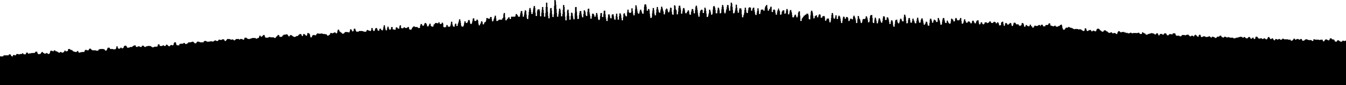
\includegraphics[width=14cm]{Methods/ImagesFils/ProfilOK.jpg}
        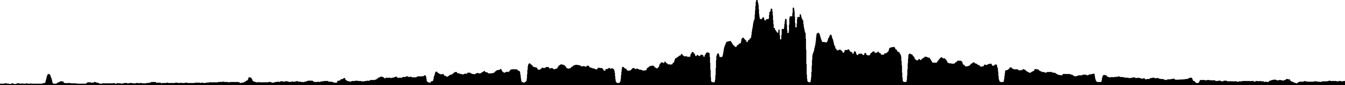
\includegraphics[width=14cm]{Methods/ImagesFils/ProfilNotOk.jpg}
        \caption{Two radiometric profil, one of a "true" wire, the other for a false positive}
\label{Fig:Line:RadiomProfil}
\end{figure}

The radiometric homogeneity if computed this way :

\begin{itemize}
   \item  a median filter is applied (size $3$) is applied,
          this low frequency filter aims at supressing the random noise,
   \item  then the total difference between the signal and convolution by a gaussian filter $\sum |I-I \circledast G| $ is computed
          to estimate the variations;
   \item  the  homogeneity is the total variation divide by the average (to have a measure
          invariant to global lighting).
\end{itemize}

This estimation of radiometric  homogeneity can be found in :

\begin{itemize}
   \item {\tt void  cParalLine::ComputeRadiomHomog(const cDataGenUnTypedIm<2> \& anIm,cPerspCamIntrCalib * aCalib,const std::string \& aNameFile)};

\end{itemize}

%-----------------------------------------------------------------------

\subsection{Selection of  \emph{best} lines}

We must now make a decision, ideally detect $1$ and only $1$ wire, but handle the case
were there is no wire, or multiple wire.


Firt if the list of candidate is not empty we consider the wire that maximize the sum of weight $SW$
defined bellow ( $\pm$ the one fitted by the maximum of points). All the other can be rejected if 
the best one is signficantly better, to see the rule used, examine the method

\begin{itemize}
   \item  {\tt bool cParalLine::RejectByComparison(const cParalLine \& aBetterOne) const;}
\end{itemize}


%-----------------------------------------------------------------------
%-----------------------------------------------------------------------
%-----------------------------------------------------------------------

\section{The \PPP command }

The command for line extraction is {\tt ExtractLine}. It takes $4$  mandatory parameters  in the following order :


\begin{itemize}
   \item  the set of images where the line must be extracted ;
   \item  a boolean indicate if the wire is white  (used when orientation of line is meaningfull like computing neighboorhouds
          or matching anti parallel line);
   \item  a folder indicating the location of an existing calibration  \footnote{it is planned to be able to use
          it w/o calibration using the key word {\tt NONE}, by the way it is still not fully working};
   \item  a folder where storing the results.
\end{itemize}

For example :

\begin{verbatim}
   MMVII ExtractLine  AllImFil.xml   true BA_311_C Fils 
   MMVII ExtractLine  (.*)_0158.tif  true BA_311_C Fils 
   MMVII ExtractLine  043_0158.tif   true BA_311_C Fils 
\end{verbatim}

For example with last command :

\begin{itemize}
    \item we will extract white line on image {\tt 043\_0158.tif};

    \item for distorsion correction we will look for intrisic calibration in 
          folder {\tt MMVII-PhgrProj/Ori/BA\_311\_/} ;

    \item the result will be stored in folder {\tt MMVII-PhgrProj/PointsMeasure/Fils};
\end{itemize}

The result will be stored in two way :

\begin{itemize}
    \item a xml file by image, that is used by \PPP ;
    \item a global file {\tt Lines.csv} that is generated for convenient use by external software.
\end{itemize}


%   -  -  -  -  -  -  -  -  -  -  -  -  -  -  -  -  -  -  -  -  -  -  -  -  -  -  -  -  -  -  -  -  -  -  -  -
% \subsubsection{AAA}








